\textbf{Входные параметры:}

 x --- входная переменная (правая граница интегрирования);
 
 Epsilon --- погрешность (например, Epsilon=0.001).

\textbf{Возвращаемое значение:}

 Значение функции в точке.
 
\textbf{Формула:}
\begin{equation*}
F\left(x \right)=\dfrac{1}{\sqrt{2\pi}}\int_0^x {e^{-\dfrac{x^2}{2}}}.
\end{equation*}

 \begin{figure} [h] 
   \center
   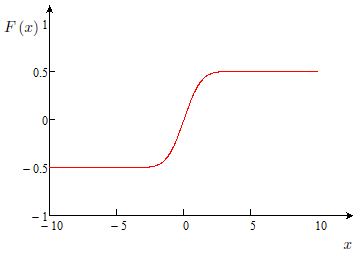
\includegraphics {MHL_DistributionFunctionOfNormalDistribution_Graph.png}
   \caption{График функции} 
   \label{img:MHL_DistributionFunctionOfNormalDistribution_Graph}  
 \end{figure}
 
